% This file was created by matlab2tikz.
%
%The latest updates can be retrieved from
%  http://www.mathworks.com/matlabcentral/fileexchange/22022-matlab2tikz-matlab2tikz
%where you can also make suggestions and rate matlab2tikz.
%
\definecolor{mycolor1}{rgb}{0.00000,0.44700,0.74100}%
%
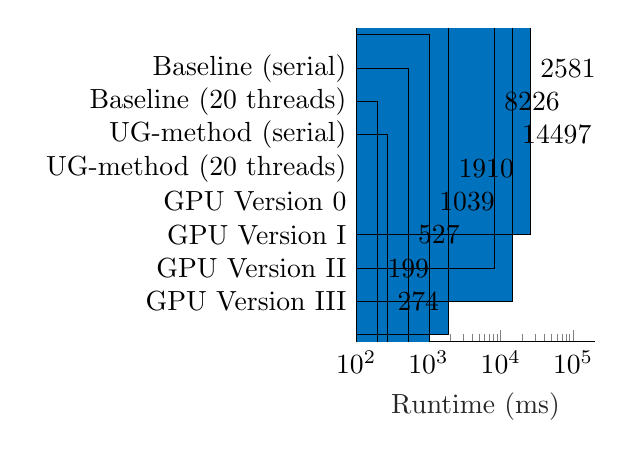
\begin{tikzpicture}

\begin{axis}[%
width=0.25\textwidth,
height=1.566in,
at={(1.637in,0.481in)},
scale only axis,
bar shift auto,
log origin=infty,
xmode=log,
xmin=100,
xmax=200000, %65817,
xminorticks=true,
xlabel style={font=\color{white!15!black}},
xlabel={Runtime (ms)},
ymin=-0.2,
ymax=9.2,
ytick={1,2,3,4,5,6,7,8},
yticklabels={{GPU Version III},{GPU Version II},{GPU Version I},{GPU Version 0},{  UG-method (20 threads)},{UG-method (serial)},{Baseline (20 threads)},{Baseline (serial)}},
axis background/.style={fill=white},
axis x line*=bottom,
axis y line*=left
]
\addplot[xbar, bar width=10, fill=mycolor1, draw=black, area legend] table[row sep=crcr] {%
274	1\\
199	2\\
527	3\\
1039	4\\
1910	5\\
14497	6\\
8226	7\\
25817	8\\
};
\node[right, align=left]
at (axis cs:274,1) {  274};
\node[right, align=left]
at (axis cs:199,2) {  199};
\node[right, align=left]
at (axis cs:527,3) {  527};
\node[right, align=left]
at (axis cs:1039,4) { 1039};
\node[right, align=left]
at (axis cs:1910,5) { 1910};
\node[right, align=left]
at (axis cs:14497,6) {14497};
\node[right, align=left]
at (axis cs:8226,7) { 8226};
\node[right, align=left]
at (axis cs:25817,8) {25817};
\end{axis}
\end{tikzpicture}%